\documentclass{article}
\usepackage[utf8]{inputenc}
\usepackage{mathtools}
\usepackage{amssymb}
\usepackage{graphicx}
\usepackage{listings}
\usepackage{float}
\usepackage{gensymb}
\usepackage{amsthm}
\usepackage{longtable}
\usepackage{adjustbox}
\usepackage{physics}
\usepackage{dsfont}
\usepackage{cancel}

\theoremstyle{definition}
\newtheorem{definition}{Definition}
\newtheorem{example}{Example}
\newtheorem{theorem}{Theorem}
\newtheorem{claim}{Claim}

\title{Quantum Information Theory}
\author{quinten tupker}
\date{January 22 2021 - \today}

\begin{document}

\maketitle

\section*{Introduction}

These notes are based on the course lectured by Professor Matthew Wingate in
Lent 2020. 
This was lectured online due to measures taken to counter the spread of Covid-19
in the UK. These are not necessarily an accurate representation of what was
lectures, and represent solely my personal notes on the content of the course,
combinged with probably, very very many personal notes and digressions... Of
course, any corrections/comments would be appreciated.

[the lecturer outlines the course] This course is an extension of the Michaelmas
Quantum Field Theory course that introduces renormalisation and the path
integral formulation of quantum field theory.

\section*{The Path Integral in Quantum Mechanics}

We start by reformulating the Schr\"{o}dinger equation as an integral equation,
which turns out to be a path integral. Anyways, starting with Schr\"{o}dinger's
equation for a Hamiltonian $H(x, p), [x, p] = i\hbar$ with

\begin{equation}
  H = \frac{p^2}{2m} + V(x)
\end{equation}

we have

\begin{equation}
  i\hbar \partial_t \ket{\psi(t)} = H \ket{\psi(t)} \implies \ket{\psi(t)} = e^{-i H t / \hbar}
  \ket{\psi(0)}
\end{equation}

where in the Schr\"{o}dinger picture the states evolve, but the operators remain
constant, and the wavefunction $\Psi(x, t) = \bra{x} \ket{\psi(t)}$. As such we
can rewrite our equation as

\begin{equation}
  \bra{x} H \ket{\psi(x)} = \left( \frac{-\hbar^2}{2m} \partial_x^2 + V(x) \right) \bra{x} \ket{\psi(t)}
\end{equation}

so we can write

\begin{align*}
  \Psi(x, t) &= \bra{x} \ket{\psi(t)} \\
             &= \bra{x} e^{-i H t / \hbar} \ket{\psi(0)} \\
             &= \int_{-\infty}^\infty dx_0 \bra{x} e^{-i H t / \hbar} \ket{x_0} \bra{x_0} \ket{\psi(0)} \\
             &= \int_{-\infty}^\infty dx_0 K(x, x_0, t) \Psi(x_0, 0)
\end{align*}

for \textbf{kernel} $K(x, x_0, t) = \bra{x} e^{-i H t / \hbar} \ket{x_0}$. Now,
if it is hard to calculate $K$ for large $t$, it can be beneficial to split this
into many intervals for many values of $t$, such as $0 = t_0 < t_1 < \dots < t_n
< t_{n + 1} = T$ leaving

\begin{equation}
  K(x, x_0, T) = \int_{-\infty}^\infty \prod_{r = 1}^n dx_r \bra{x_{r + 1}} e^{- iH(t_{r + 1} - t_r) / \hbar} \ket{x_r} \bra{x_1} e^{-iH (t_1 - t_0) / \hbar} \ket{0}
\end{equation}

which is in a sense an integral over all possible sequences of values of $x$. 

In free field theory ($V = 0$) this can be explicitly evaluated using a Gaussian
integral by rewriting things in the momentum basis as (use $\bra{x} \ket{p} =
e^{i px / \hbar}$)

\begin{align*}
  K_0(x, x', t) &= \bra{x} e^{\frac{-i p^2 t}{2m \hbar}} \int \frac{dp}{2\pi \hbar} \ket{p} \bra{p} \ket{x'} \\
                &= \int_{-\infty}^\infty \frac{dp}{2 \pi \hbar} e^{\frac{-ip^2 t}{2m \hbar}} e^{ip (x - x') / \hbar}\\
                &= e^{\frac{ip(x - x')^2}{2\hbar t}} \sqrt{\frac{m}{2\pi i \hbar t}}
\end{align*}

where we note that the limit as $t \to 0$ is $\delta(x - x')$ which indeed
matches $\bra{x} \ket{x'} = \delta(x - x')$ as expected.

Now in an interacting theory, we struggle with the Baker-Campbell-Hausdorff fact
that $e^A e^B \neq e^{A + B}$ so using Suzuki-Trotter we separate into steps
size $t_{r + 1} - t_r = \delta t << T$ meaning that

\begin{equation}
  e^{-iH \delta t / \hbar} \approx e^{\frac{-ip^2 \delta t}{2m \hbar}} e^{\frac{-i V(x) \delta}{\hbar}} (1 + O(\delta t^2))
\end{equation}

so for $T = n \delta t$ we find that

\begin{equation}
  K(x, x_0, T) = \int \prod_{r = 1}^n dx_r \left( \frac{m}{2\pi i \hbar \delta t} \right)^{\frac{n + 1}{2}}
  e^{i \sum_{r = 0}^n \left( \frac{m}{2 \hbar} \left( \frac{x_{r + 1} - x_r}{\delta t} \right)^2
      - V(x_r) / \hbar \right) \delta t}
\end{equation}

which in the limit $n \to \infty, \delta t \to 0$ while keeping $T$ constant
leaves

\begin{equation}
  \frac{1}{\hbar} \int_0^T dt \left( \frac{1}{2}m \dot{x}^2 - V(x) \right) = \int_0^T dt L(x, \dot{x}) = S
\end{equation}

for classical Lagrangian $L$ and action $S$. This is what we refer to as a path
integral or function integral:

\begin{equation}
  K(x, x_0, t) = \int \mathcal{D}x e^{i S / \hbar}
\end{equation}

where $\mathcal{D} x$ is the limit describd above. Of course, many questions
about the existence and uniqueness, etc. of such limits exists, and in fact
often this limit does not exist, but in the cases we are interested it, it works
well enough... [End of lecture 1]

We make the following remarks

\begin{itemize}
\item In the classical limit $\hbar \to 0$ the lowest frequencies
  dominate $K$. This is equivalent to Hamilton's principle (the principle of
  least action), as expected.
\item it is common and helpful to extend analytically to imaginary time $\tau =
  it$ leaving $\bra{x} e^{-H\tau / \hbar} \ket{x_0} = \int \mathcal{D}x e^{-S /
    \hbar}$ which has better convergence properties and is easier to interpret
  than the complex version (Hamilton's principle appears more easily as well). 
\end{itemize}

\section{Integrals and their diagrammatic expansion}

The above considered quantum mechanics, which is in a sense the $0 + 1$
dimension vrsion of QFT (since $x$ is treated as an operator, while $t$ is
treated as a variable). To move to more general QFT, we start, strangely, with 0
dimensional QFT, for $\phi : \{ \cdot \} \to \mathbb{R}$ a field on a single
point. Here,

\begin{equation}
  \mathcal{Z} = \int_\mathbb{R} d\phi e^{-S(\phi) / \hbar}
\end{equation}

where we assume $S$ is an even polynomial in $\phi$ for convergence reasons, and
we are interested in expectation values

\begin{equation}
  \langle f \rangle = \frac{1}{\mathcal{Z}} \int d\phi f(\phi) e^{-S(\phi) / \hbar}
\end{equation}

\subsection{Free Theory}

For $N$ fields $\phi_a, a = 1, \dots, N$, let $S(\phi) = \frac{1}{2} \phi^T m
\phi$ for a symmetric positive definite matrix $m = P\Delta P^T$ for orthogonal
$P$. As such, we can write this essentially Gaussian integral as

\begin{equation}
  \mathcal{Z}_0 = \int d^N \phi e^{-\frac{1}{2 \hbar} \phi^T m \phi} = \sqrt{\frac{(2\pi\hbar)^N}{\det m}}
\end{equation}

From here, we can turn this into a generating function to calculate expectation
values by taking derivatives by turning $S_0(\phi) \mapsto S_0(\phi) - J^T
\phi$, and writing $\mathcal{Z}_0 = \mathcal{Z}_0(J)$ (now a generating
function(al) - functional later on). We then remark

\begin{equation}
  \mathcal{Z}_0(J) = \mathcal{Z}_0(0) e^{-\frac{1}{2\hbar} J^T m^{-1} J}
\end{equation}

Then we can calculate the correlation functions as

\begin{equation}
  \langle \phi_a \phi_b \rangle = \frac{1}{Z_0(0)} \hbar^2 \partial_{J_a} \partial_{J_b} \mathcal{Z}_0(J) |_{J = 0}
  = h(m^{-1})_{ab}
\end{equation}

Conveniently, this can be diagrammatically interpreted as a connecting two
vertices on indices $a, b$ with an undirected edge. We can generalise this to
linear operator $l(\phi) = \sum l_a \phi_a$ as (for $p$ such operators)

\begin{equation}
  \langle l^{(1)}(\phi) \dots l^{(p)}(\phi) \rangle = \hbar^p \prod_{i = 1}^p l^{(i)}(\partial_J) e^{\frac{1}{\hbar} J^T m^1 J}
\end{equation}

If $p$ is odd, this is always 0 by symmetry, but if $p$ is even this corresponds
to a linear combination of products $m_{ab}^{-1} m_{cd}^{-1} \dots$

\begin{example}
  For $p=4, l^{(1)}_a = \delta_{ab}, l^{(2)}_a = \delta_{ac}, l^{(3)}_a =
  \delta_{ad}, l^{(4)}_a = \delta_{af}$ then
  \begin{equation}
    \langle \phi_b \phi_c \phi_d \phi_f \rangle = \hbar^2 (m_{bc}^{-1} m_{df}^{-1} + m_{bd}^{-1} m_{cf}^{-1} +
    m_{bf}^{-1} m_{cd}^{-1})
  \end{equation}
  which also corresponds to the ways in which we can connect four vertices with
  undirected edges
  \begin{figure}[H]
    \centering
    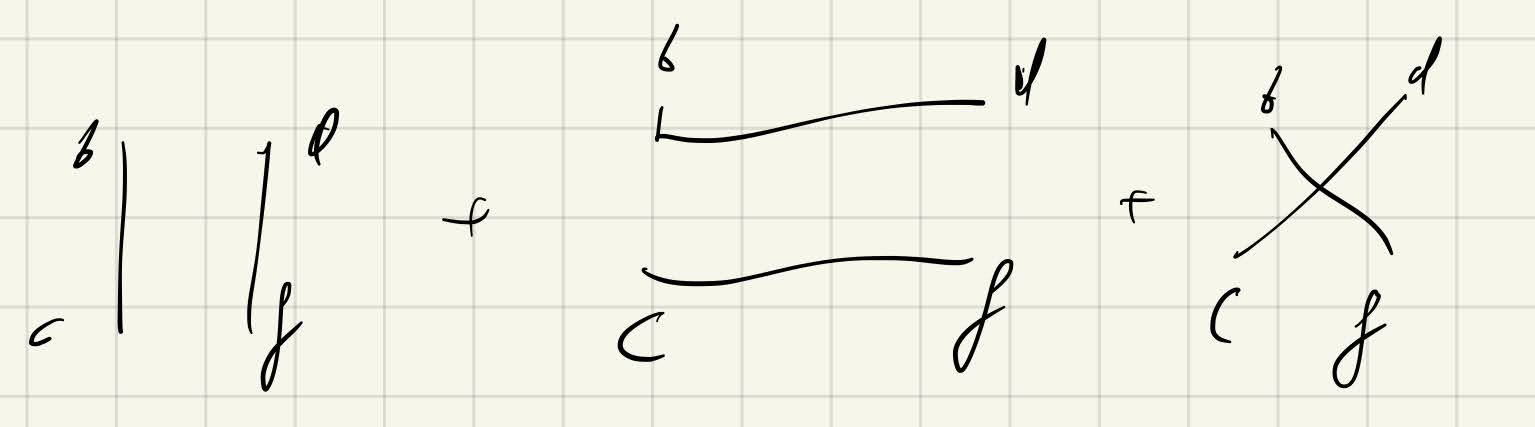
\includegraphics[width=7cm]{res/AQFT/connecting_four_vertices}
    \label{connecting_four_vertices}
  \end{figure}
\end{example}

[End of lecture 2]

\subsection{Interacting Theory}

We start investigating interacting theory by doing a series expansion of

\begin{equation}
  \int_{\mathbb{R}^N} \d^N \phi f(\phi) e^{-S / \hbar}
\end{equation}

in $\hbar$. However, we find that in general, the radius of convergence of these
perturbed series is 0, since if we take $\hbar < 0$ these do not converge. As
such, we get asymptotic behaviour along the lines described by saying that

\begin{definition}
  $I(\hbar)$ is \textbf{asymptotic} to $\sum_{n = 0}^\infty c_n \hbar^n$
  (denoted by $\sim$) if $\lim_{\hbar \to 0^+} \frac{1}{\hbar^N} | I(\hbar) -
  \sum_{n = 0}^N c_n \hbar^n | = 0$ for fixed $N$.
\end{definition}

This is much weaker than convergence since we find that adding new terms may in
fact make things worse. But it does allow us to account for transcendental terms
like $e^{-1 / \hbar^2} ~ 0$ (called \textbf{nonperturbative contributions}).

Now we work out the case where

\begin{equation}
S(\phi) = \frac{1}{2} m^2 \phi^2 + \frac{\lambda}{4!} \phi^4
\end{equation}

and expand about the minimum of $S$ at $\phi=0$ to get

\begin{equation}
\mathcal{Z} = \int d\phi e^{-S / \hbar} = \int d\phi e^{-S / \hbar} 
\sum_v^\infty \frac{1}{v!} \left( \frac{-\lambda}{4! \hbar} \phi^4 \right)^v
\end{equation}

but since we don't converge, we certainly can't swap $\int$ and $\sum$ so here
we first truncate, and then swap. As such, if we write $x = \frac{1}{2\hbar} m^2
\phi^2$,

\begin{equation}
\mathcal{Z} \sim \frac{\sqrt{2\hbar}}{m} \sum_{v = 0}^N \frac{1}{v!} \left( 
\frac{-\hbar \lambda}{4! m^4} \right)^v 2^{2v} \int_0^\infty dx e^x x^{2v
+ 1/2 - 1}
\end{equation}

where the integral is just the gamma function $\Gamma(2v + 1/2) = \frac{(4v)!
  \sqrt{\pi}}{4^{2v} (2v)!}$ so

\begin{equation}
\mathcal{Z} \sim \frac{\sqrt{2\hbar}}{m} \sum_{v = 0}^N \frac{1}{v!} \left( 
\frac{-\hbar \lambda}{4! m^4} \right)^v \frac{1}{(4!) v} \frac{(4v)! \sqrt{\pi}}{2^{2v} (2v)!}
\end{equation}

(the lecture notes seem to omit the $\sqrt{\pi}$). Here the $\frac{1}{(4!) v}$
comes from expanding the interaction term $e^{-S_1 / \hbar}$ and the second
fraction comes from the number of ways to pair $4v$ fields with $v$ copies of
$\phi^4$. Applying stirling's formula, this series grows as $v!$ so this series
is definitely not convergent, but still asymptotic. Now, as before, we want to
insert our $J$ somehow to get a generating function. Here we get

\begin{align*}
\mathcal{Z}(J) &= \int d\phi e^{-\frac{1}{\hbar} (S_0(\phi) + S_1(\phi) - J\phi)} \\
&= e^{-\frac{1}{\hbar} S_1(\hbar \partial_J)} \int d\phi e^{-\frac{1}{\hbar} 
(S_0(\phi) - J\phi)} \\
&\sim e^{-\frac{\lambda}{4! \hbar} (\hbar \partial_J)^4} e^{\frac{1}{2\hbar} J^T m^{-1} J}
\end{align*}

which works out to

\begin{equation}
  \mathcal{Z}(J) \sim \sum_{v=0}^N \frac{1}{v!} \left( \frac{-\lambda}{4! \hbar}
    (\hbar \partial_J)^4 \right)^v \sum_{p = 0} \frac{1}{p!} \left( \frac{1}{2\hbar}
    J^T m^{-1} J \right)^p
\end{equation}

where diagramatically $v$ corresponds to the number of vertices, and $p$ to the
number of propagators.

\begin{figure}[H]
  \centering
  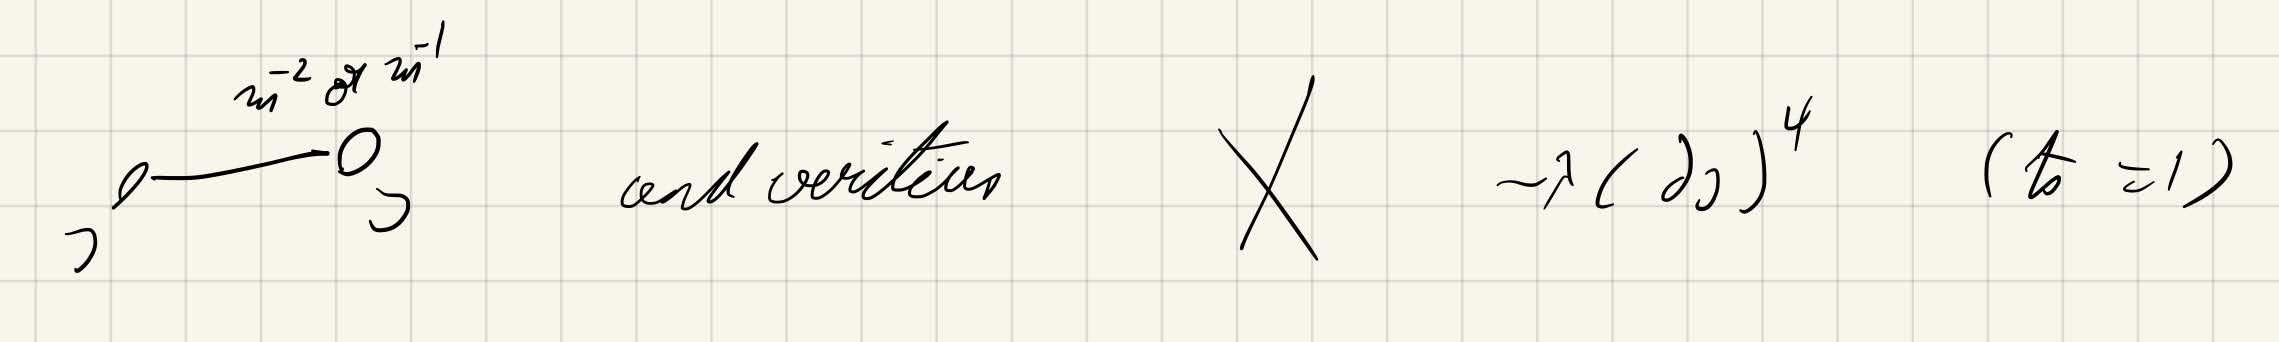
\includegraphics[width=7cm]{res/AQFT/diagram_interpretation}
  \label{diagram_interpretation}
\end{figure}
 
where in order to get a nonzero term we need the number of derivatives ($4v$
vertex line ends - 4 per vertex here) to match the number of sources ($2p$ for
each propagator) to match. However, we can have a predetermined number of
external sources $E = 2p - 4v$. For example, the first two nontrivial terms in
the $Z(0)$ expansion for $E = 0$ are $(v, p) = (1, 2), (2, 4)$ which corresponds
diagrammatically to

\begin{figure}[H]
  \centering
  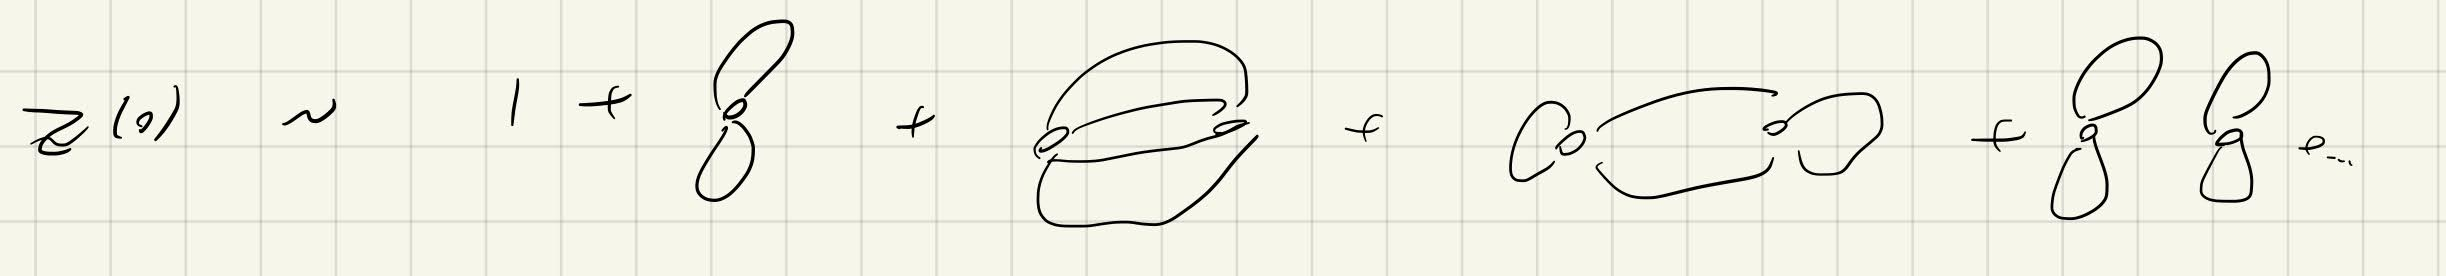
\includegraphics[width=7cm]{res/AQFT/quartic_series_diagram}
  \label{quartic_series_diagram}
\end{figure}

Note that each diagram may have a factor in front of it determined by how often
it repeats itself (affect by the product rule in taking derivatives). [end of
lecture 3]

\end{document}